\section{Korrelationen zwischen Städten und ihrem Umland}
In \autoref{fig:highest_selected_counties} sind die Korrelationswahrscheinlichkeiten zwischen den in Abschnitt \autoref{} beschrieben Städten und den Landkreisen für eine zeitliche Verschiebung zwischen $\tau=-50$ und $\tau=50$ als Kurven dargestellt.
\todo{Städte und Landkreisnamen verlinken}
Die Kurven, deren Höhepunkt rechts der null sind, sind rot eingefärbt. Die Kurven mit dem höchsten Punkt links der null sind blau gefärbt. Die restlichen Kurven, welche am Nullpunkt maximal werden, sind grün gefärbt.
\begin{figure}[H]
    \centering
    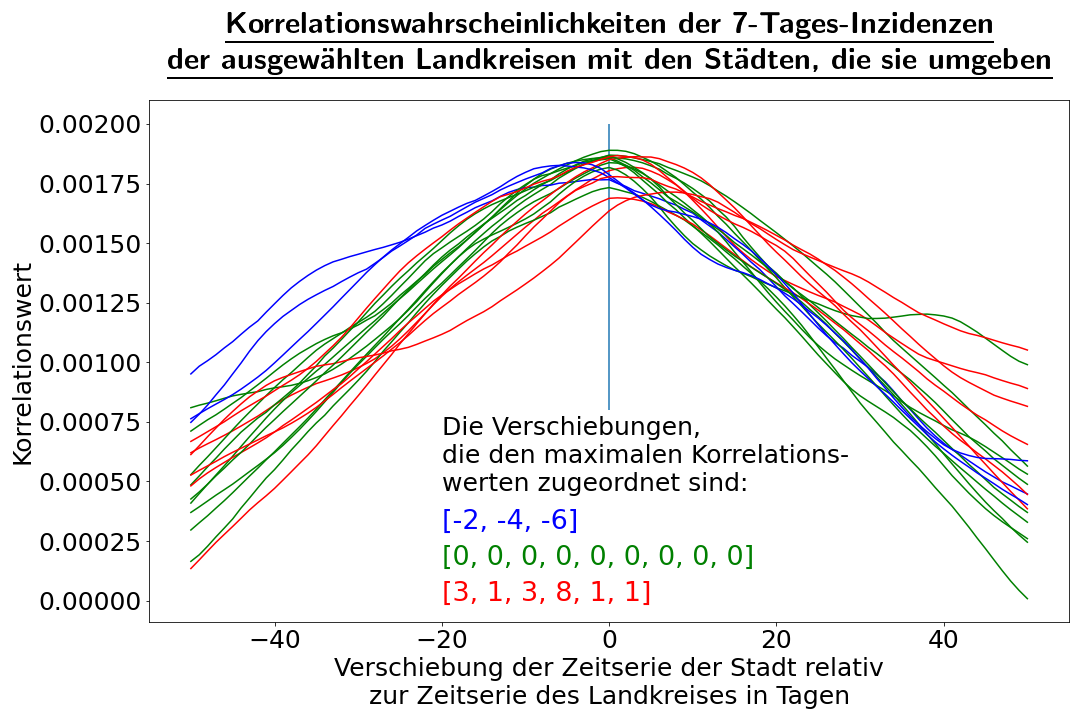
\includegraphics[width = 0.95\textwidth]{figures/Ergebnisse/highest_selected_counties.png}
    \caption{Die Korrelationswahrscheinlichkeiten der 7-Tages INzidenzen der ausgewählten Landkreise mit den Städten, die sie umgeben. Die Kurven sind je nach ihrem Hochpunkt eingefärbt: Rot bei positiven x-Werte, Blau bei negativen und grün bei 0.}
    \label{fig:highest_selected_counties}
\end{figure}

In dieser sehr kleinen Teilmenge weißen 50~\% der Korrelationen die höchste Korrelationswahrscheinlichkeit bei einer Verschiebung von $\tau = 0$ auf.
Bei den Korrelationen aller deutschen Landkreise untereinander liegt bei 8,7~\% die höchste Korrelationswahrscheinlichkeit bei einer Verschiebung von $\tau= 0$ (8,5~\% wenn man die Autokorrelationen herausrechnet).

Abbildung \autoref{fig:sum_selected_counties} zeigt die Differenz zwischen der durchschnittlichen Korrelationswahrscheinlichkeit für negative Verschiebungen und derdurchschnittlichen Korrelationswahrscheinlichkeit für positive Verschiebungen.
\begin{figure}
    \centering
    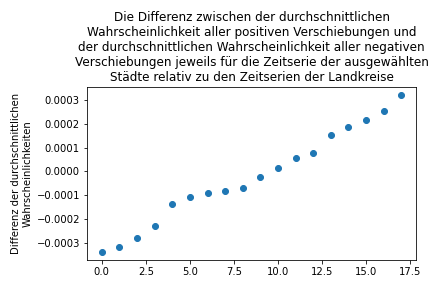
\includegraphics[width=0.95\textwidth]{figures/Ergebnisse/sum_selected_counties.png}
    \caption{Die Differenz zwischen der durchschnittlichen Korrelationswahrscheinlichkeit aller negativen Verschiebungen und der durchschnittlichen Korrelationswahrscheinlichkeit aller positiven Verschiebungen für die ausgewählten Korrelationen zwischen Städten und Landkreisen.}
    \label{fig:sum_selected_counties}
\end{figure}